% Copyright 2004 by Till Tantau <tantau@users.sourceforge.net>.
%
% In principle, this file can be redistributed and/or modified under
% the terms of the GNU Public License, version 2.
%
% However, this file is supposed to be a template to be modified
% for your own needs. For this reason, if you use this file as a
% template and not specifically distribute it as part of a another
% package/program, I grant the extra permission to freely copy and
% modify this file as you see fit and even to delete this copyright
% notice. 

\documentclass{beamer}
\usepackage{subcaption}

\captionsetup{compatibility=false}
% Replace the \documentclass declaration above
% with the following two lines to typeset your 
% lecture notes as a handout:
%\documentclass{article}
%\usepackage{beamerarticle}


% There are many different themes available for Beamer. A comprehensive
% list with examples is given here:
% http://deic.uab.es/~iblanes/beamer_gallery/index_by_theme.html
% You can uncomment the themes below if you would like to use a different
% one:
%\usetheme{AnnArbor}
%\usetheme{Antibes}
%\usetheme{Bergen}
%\usetheme{Berkeley}
%\usetheme{Berlin}
%\usetheme{Boadilla}
%\usetheme{boxes}
%\usetheme{CambridgeUS}
%\usetheme{Copenhagen}
%\usetheme{Darmstadt}
%\usetheme{default}
%\usetheme{Frankfurt}
\usetheme{Goettingen}
%\usetheme{Hannover}
%\usetheme{Ilmenau}
%\usetheme{JuanLesPins}
%\usetheme{Luebeck}
%\usetheme{Madrid}
%\usetheme{Malmoe}
%\usetheme{Marburg}
%\usetheme{Montpellier}
%\usetheme{PaloAlto}
%\usetheme{Pittsburgh}
%\usetheme{Rochester}
%\usetheme{Singapore}
%\usetheme{Szeged}
%\usetheme{Warsaw}

\title{Final Evaluation}

% A subtitle is optional and this may be deleted
\subtitle{LELEC2103}

\author{Bronchain Olivier \and Schellekens Vincent}
% - Give the names in the same order as the appear in the paper.
% - Use the \inst{?} command only if the authors have different
%   affiliation.

\institute[Ecole Polytechnique de Louvain]{
    Ecole Polytechnique de Louvain} % (optional, but mostly needed)

% - Use the \inst command only if there are several affiliations.
% - Keep it simple, no one is interested in your street address.

\date{\today}
% - Either use conference name or its abbreviation.
% - Not really informative to the audience, more for people (including
%   yourself) who are reading the slides online

% This is only inserted into the PDF information catalog. Can be left
% out. 

% If you have a file called "university-logo-filename.xxx", where xxx
% is a graphic format that can be processed by latex or pdflatex,
% resp., then you can add a logo as follows:

% \pgfdeclareimage[height=0.5cm]{university-logo}{university-logo-filename}
% \logo{\pgfuseimage{university-logo}}

% Delete this, if you do not want the table of contents to pop up at
% the beginning of each subsection:
\AtBeginSubsection[]
{
  \begin{frame}<beamer>{Outline}
    \tableofcontents[currentsection,currentsubsection]
  \end{frame}
}

% Let's get started
\begin{document}

\begin{frame}
  \titlepage
\end{frame}

\begin{frame}{Outline}
  \tableofcontents
  % You might wish to add the option [pausesections]
\end{frame}

\section{Frame detection \& Frequency Offset Correction}
\subsection{Objectives and method}
\begin{frame}{Frame detection \& frequency offset correction : what for?}
    \begin{itemize}
    \item Goal of frame detection : locate the beginning of the frame despite the signal suffering an unknown delay
    \item Goal of frequency offset correction : even small $\Delta f$ at $Tx$ and $Rx$ $\Rightarrow$ distortions that need to be corrected
    \end{itemize}
    We will (again) use \textit{training sequences} to do these operations
\end{frame}

\begin{frame}{Frame detection by correlation}
    Idea : use a training sequence with strong \textit{autocorrelation} properties
\end{frame}



\subsection{Practical results}


%%% CACA 
% GROS PD
% Je nique ta ... soeur/mère , vu que c'est les deux en même temps #consanguin
% Je nique tes fesses
% Du coup c'est toi le gros PD 
% CQFD
% ouais mais t'aimes ça$
% cochon
% J'vais balancer à Anso 
% du gros son


\section{OFDM}
\subsection{Narrowband vs wideband channels}

\begin{frame}{Narrowband vs wideband channels}
    To use a narrowband channel we take:
        \begin{itemize}
        \item Sample rate: $4M Sample/s$
        \item Oversampling factor: $20$
        \item Bandwidth: $0,1 MHz$
        \end{itemize}
    To use a wideband channel we take:
        \begin{itemize}
        \item Sample rate: $20M Sample/s$
        \item Oversampling factor: $4$
        \item Bandwidth: $2.5 MHz$
        \end{itemize}
\end{frame}
\begin{frame}{Power delay}
                \begin{figure}[h!]
                    \centering
                    \begin{subfigure}[b]{0.45 \textwidth}
                        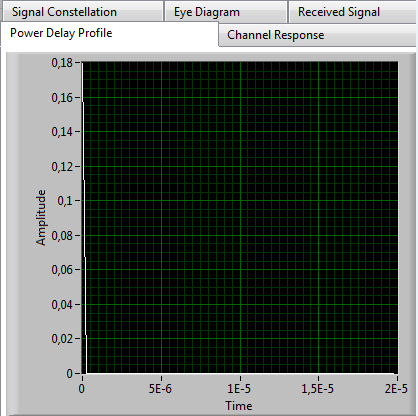
\includegraphics[width=\textwidth]{narrowT.PNG}
                        \caption{Narrowband channel}\label{fig:2}
                    \end{subfigure}
                    ~
                    \begin{subfigure}[b]{0.45 \textwidth}
                   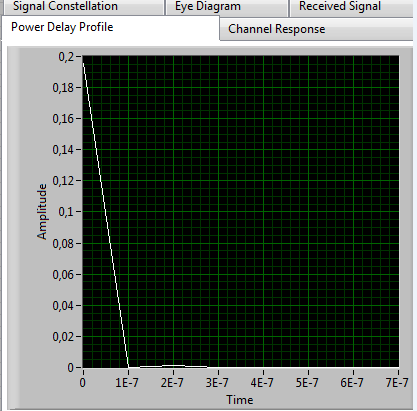
\includegraphics[width=\textwidth]{wideT.PNG}
                        \caption{Wideband channel}\label{fig:4}
                    \end{subfigure}
                    \caption{Power delay}\label{fig:const}
                \end{figure}
\end{frame}


\begin{frame}{Channel frequency response}
                \begin{figure}[h!]
                    \centering
                    \begin{subfigure}[b]{0.45 \textwidth}
                        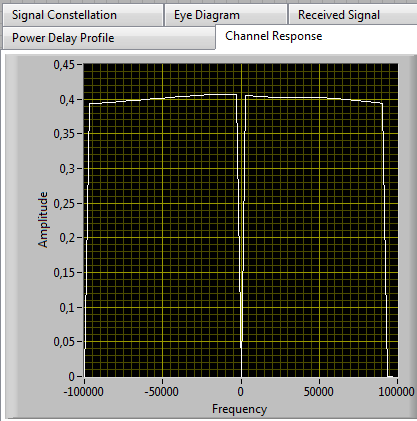
\includegraphics[width=\textwidth]{narrowRep.PNG}
                        \caption{Narrowband channel}\label{fig:2}
                    \end{subfigure}
                    ~
                    \begin{subfigure}[b]{0.45 \textwidth}
                   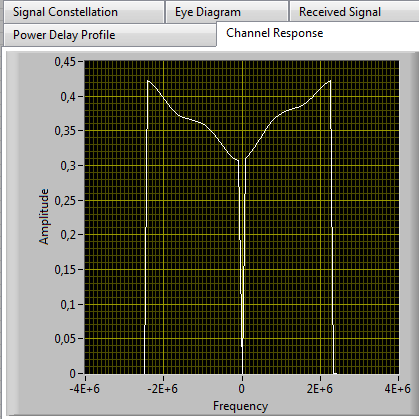
\includegraphics[width=\textwidth]{wideRep.PNG}
                        \caption{Wideband channel}\label{fig:4}
                    \end{subfigure}
                    \caption{Channel frequency response}\label{fig:const}
                \end{figure}
\end{frame}

\begin{frame}{Narrowband vs wideband channels}
    We can observe that:
	\begin{itemize}
		\item A Narrowband channel is flat because $L_h=0$
		 	$$ H[k] = \sum_{l=0}^{L_h} e^{-j2\pi kl/N} = h[0]e^{-j2\pi kl/N} = h[0] \forall k$$
		\item A Wideband channel is frequency selective because $L_h > 0$.
	
		$$ k_1 = 0 \quad and \quad k_2 = N/2$$
			$$ H[k_1] = \sum_{l=0}{L_h} h[l] \quad and \quad H[k_2] = \sum_{l=0}{L_h}(-1)^lh[l]$$
			$$ H[k_1] \neq H[k_2] $$
	\end{itemize}
\end{frame}

\subsection{OFDM overview}
\begin{frame}{OFDM overview}
	We want to transfer $\{s[n]\}_{n=0} ^{N-1}$ where N is the number of subcarriers. We transfer in time domain:
	\begin{align*}
		w[n] 	&= iDFT(s[m]) \\ 
			&=\frac{1}{N} \sum_{m=0}^{N-1} s[m] e^{j 2 \pi \frac{m(n-L_c)}{N}} \quad  n=0,..., N+L_c-1
	\end{align*}
	Due to channel response we receive signal:
	$$\overline{y}[n] = \sum_{l=0}^{L} h[l]w[n-l]+v[n]$$
	His DFT gives:
	\begin{align*} 
		\overline{Y}[k] &= DFT[\overline{y}[n]]\\
			& = H[k]s[k]+V[k]
	\end{align*}
\end{frame}

\subsection{Sensitivity to frequency offset}
    
\begin{frame}{Frequency offset influence}
                \begin{figure}[h!] 
 	                \centering
                       	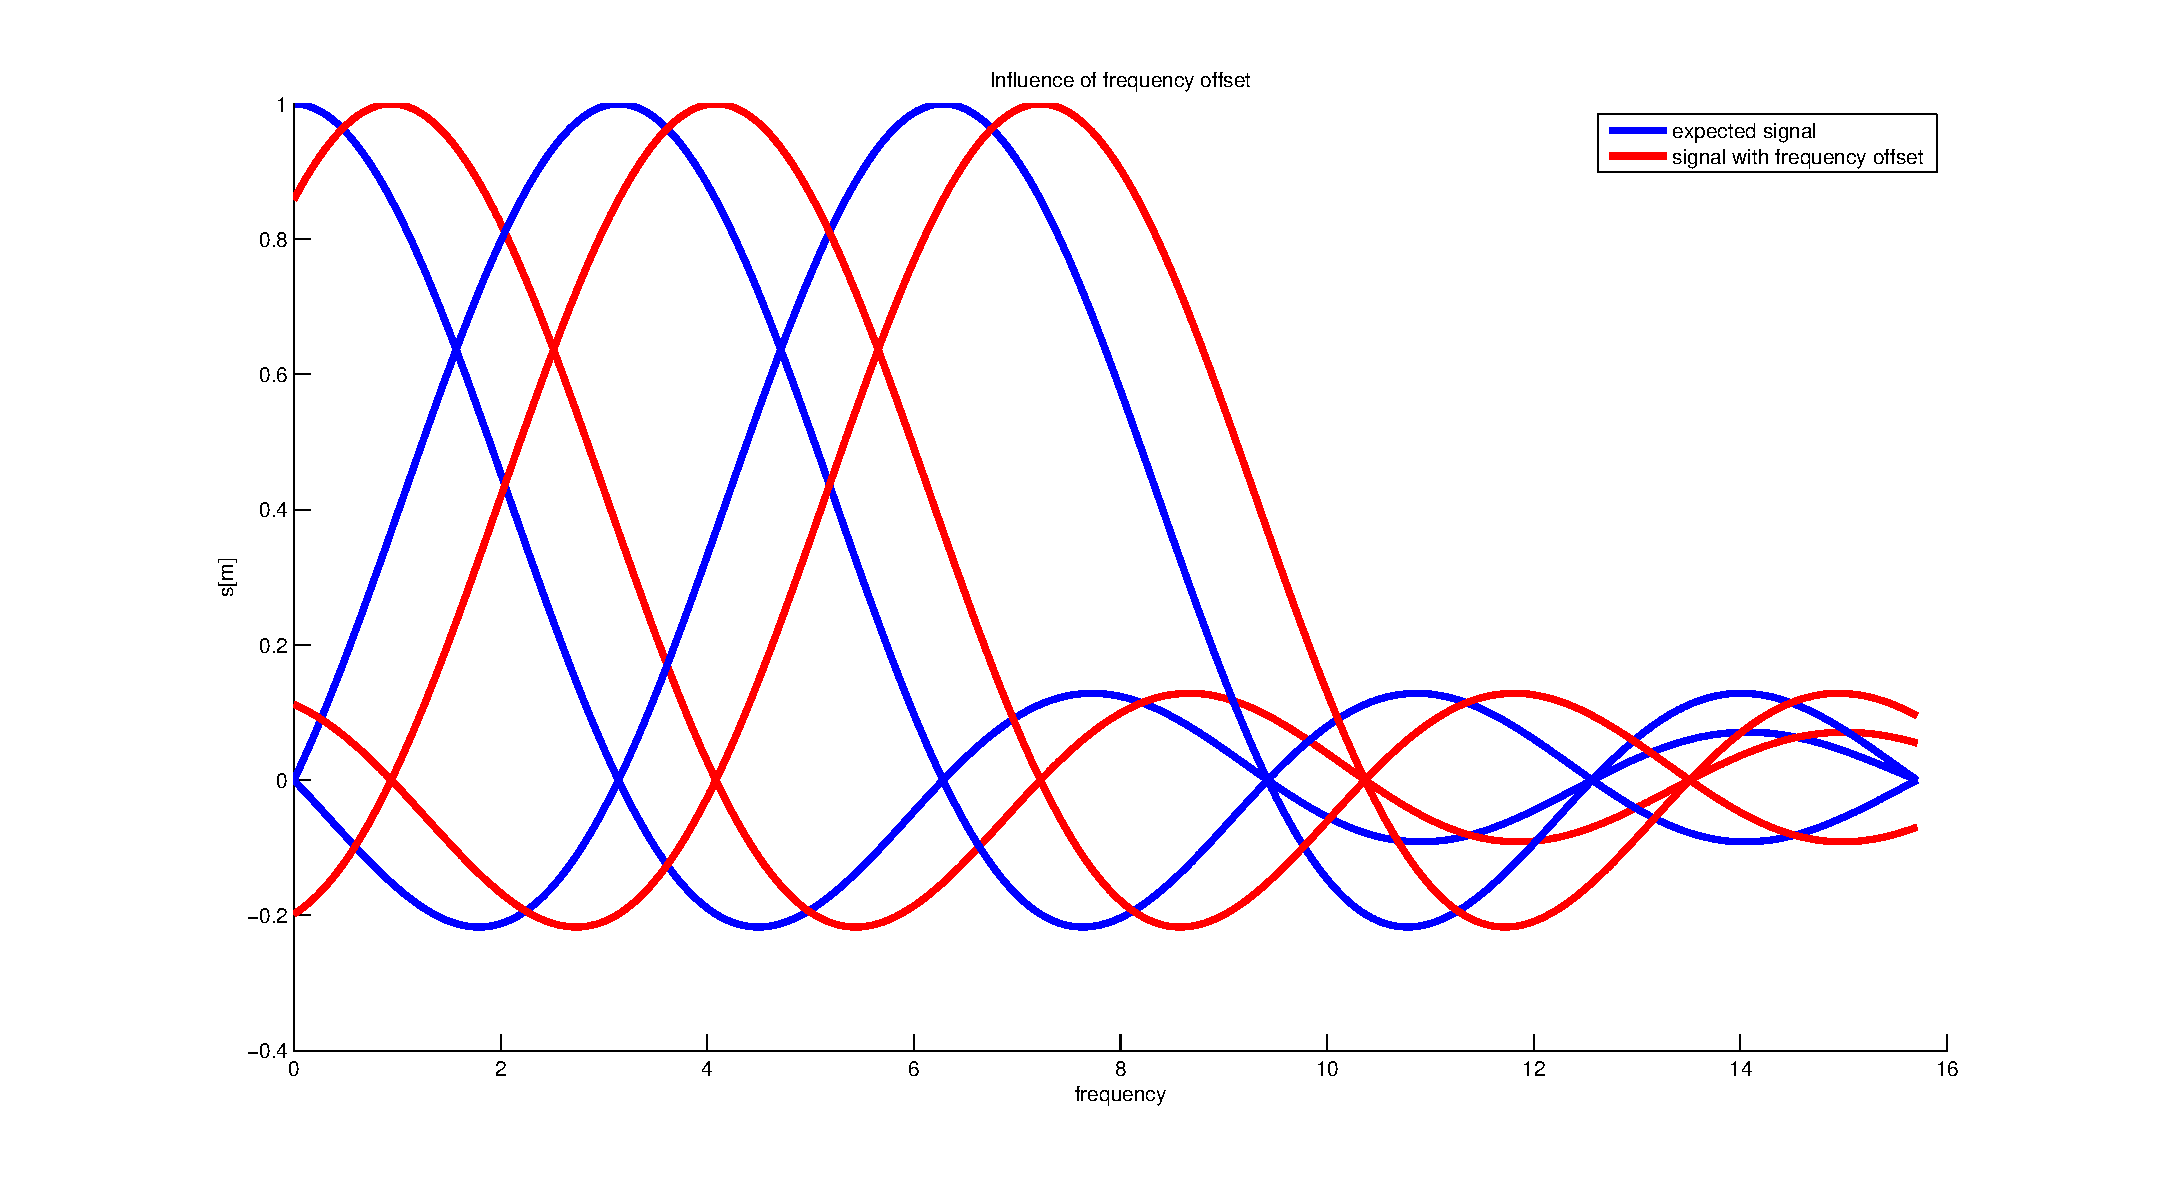
\includegraphics[width= 0.8\textwidth]{frequencyInf.eps}
                \end{figure}
		\begin{figure}[h!]
			\centering
			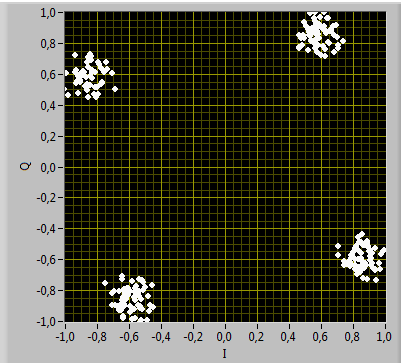
\includegraphics[width= 0.3\textwidth]{off50_1024.PNG}
			\caption{Influence of frequency offset in OFDM}
		\end{figure}
\end{frame}

\begin{frame}{Number of subcarriers influence}
	What happen  when the number of subcarriers grows ?
	\begin{itemize}
		\item There is more subcarriers for a certain bandwidth
		\item Less resistant against frequency offset
	\end{itemize} 
		\begin{figure}[h!]
			\centering
			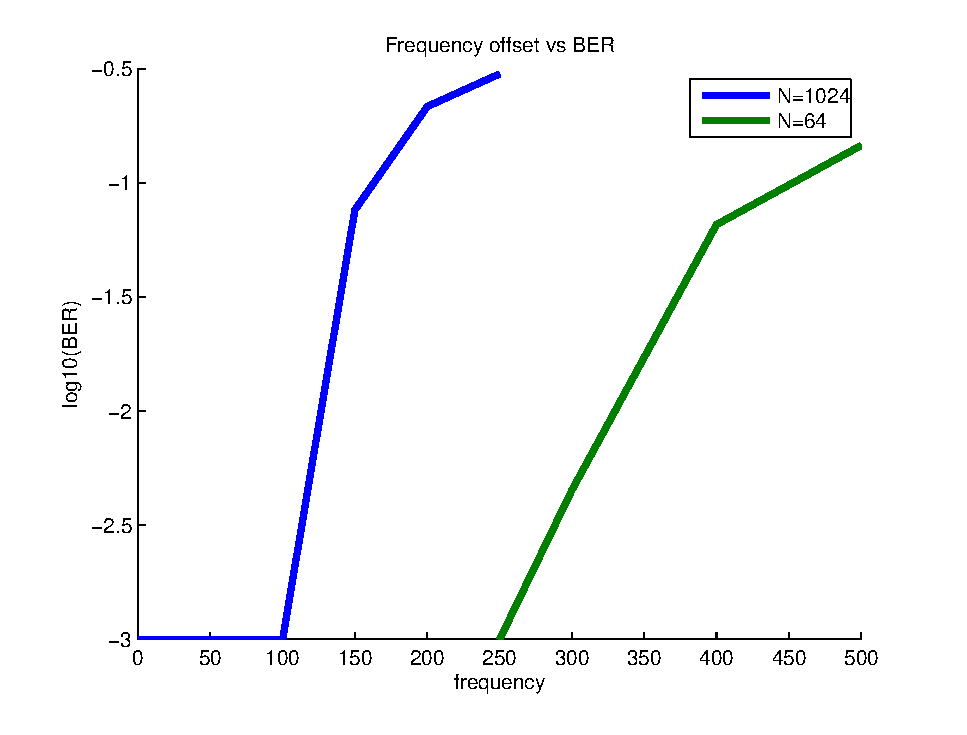
\includegraphics[width = 0.65\textwidth]{fber.eps}
			\caption{BER vs frequency offset for different subcarriers}
		\end{figure}	
\end{frame}

\subsection{Parameters of a OFDM modulation}
\begin{frame}{Parameters of a OFDM modulation}
	We can choose at least 3 parameters for a OFDM modulation:	
	\begin{itemize}
		\item Increasing the number of subcarriers:
			\begin{itemize}
				\item Make the channel less frequency selective
				\item Increase OFDM frequency offset sensibility
			\end{itemize}
		\item Increasing the bandwith
			\begin{itemize}
				\item Make the channel more frequency selective
				\item Decrease OFDM frequency offset sensibility
			\end{itemize}
		\item The length of the cyclic prefix
			\begin{itemize}
				\item Avoid ICI
				\item Should be at least greater then $L_h$
			\end{itemize}
	\end{itemize}
\end{frame}

\end{document}
